%\postdisplaypenalty =1000

\chapter{Sistemi a tempo continuo}

	\begin{definizione}
		\textbf{un sistema dinamico} è un modello matematico che rappresenta un oggetto con un numero finito di gradi di libertà che evolve nel tempo secondo  una legge deterministica
	\end{definizione}
	\subsubsection{Esempi semplici}
		\begin{nexample}
			Il pendolo è un esempio semplice di sistema che ha come input la gravità e come output la posizione x nel tempo.
			Questo sistema è stabile perchè il pendolo tende a tornare nella posizione di equilibrio.
			
			\begin{figure}[H]
				\centering
				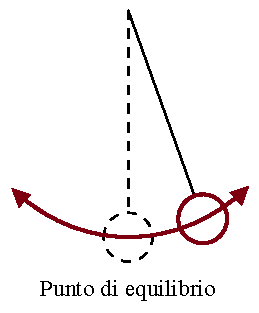
\includegraphics[scale=0.25]{immagini/cap3_Sistemi/pendolo}
				\caption{ Sistema semplice: pendolo. }
				\label{fig: pendolo}
			\end{figure}
			
			\begin{figure}[H]
				\centering
				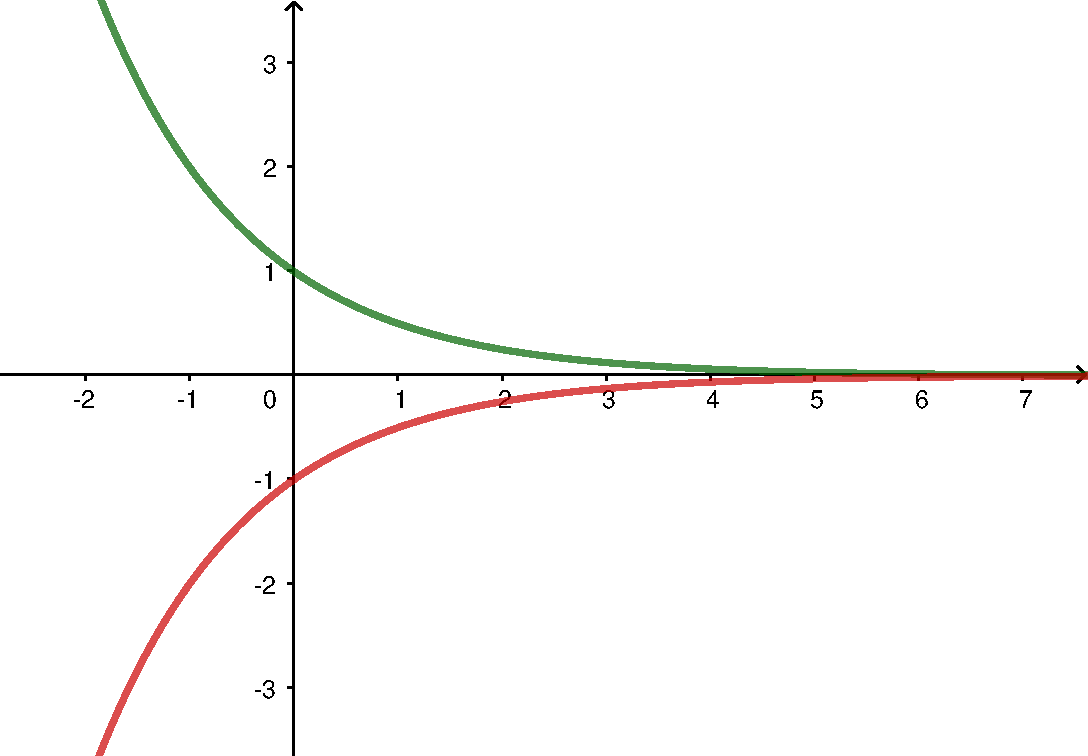
\includegraphics[scale=0.5]{immagini/cap3_Sistemi/sistEquilib.pdf}
				\caption{ Grafico che descrive l'andamento nel tempo del pendolo, come si può vedere tende a zero infatti il sistema è in equilibrio. }
				\label{fig: funzpendolo}
			\end{figure}
			
		\end{nexample}

%%\pagebreak

	\begin{nexample}
			Una palla che cade in una buca è un altro esempio di sistema stabile, l'input è sempre la gravità e la posizione x è l'output. 
%			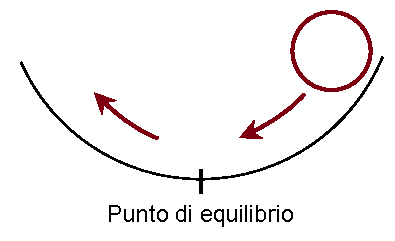
\includegraphics[scale=0.5]{immagini/cap3_Sistemi/pallaBuca.pdf}
%			\caption{ Sistema semplice: palla che cade in una buca. }		
		\begin{figure}[H]
			\centering
			\subfloat[][\emph{Palla che cade in una buca}]
			{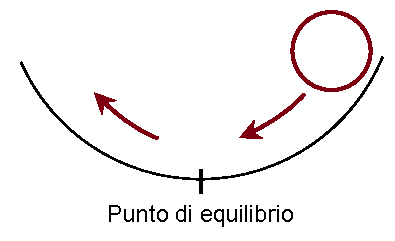
\includegraphics[width=.45\textwidth]{immagini/cap3_Sistemi/pallaBuca.pdf}} \quad
			\subfloat[][\emph{Grafico che descrive l'andamento della palla, come si può vedere tende a zero infatti il sistema è in equilibrio.}]
			{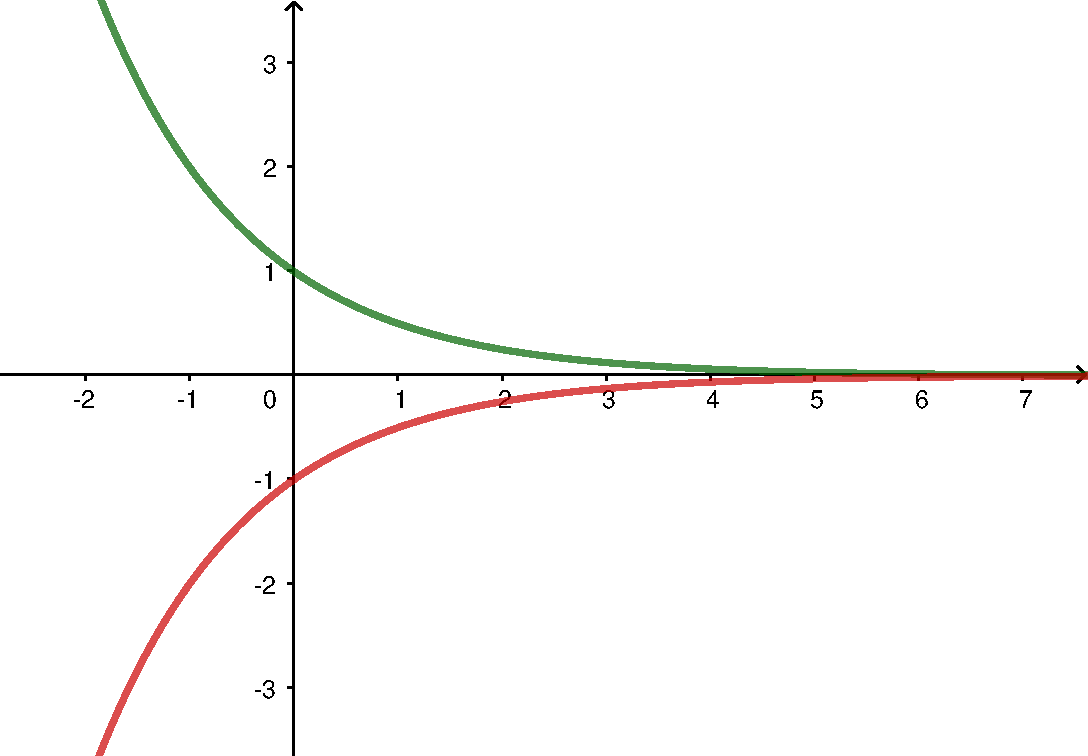
\includegraphics[width=.45\textwidth]{immagini/cap3_Sistemi/sistEquilib.pdf}} 
			\caption{ Sistema semplice: palla che cade in una buca. }
			\label{fig: pallaBuca}
		\end{figure}
		
%		\begin{figure}[H]
%			\centering
%			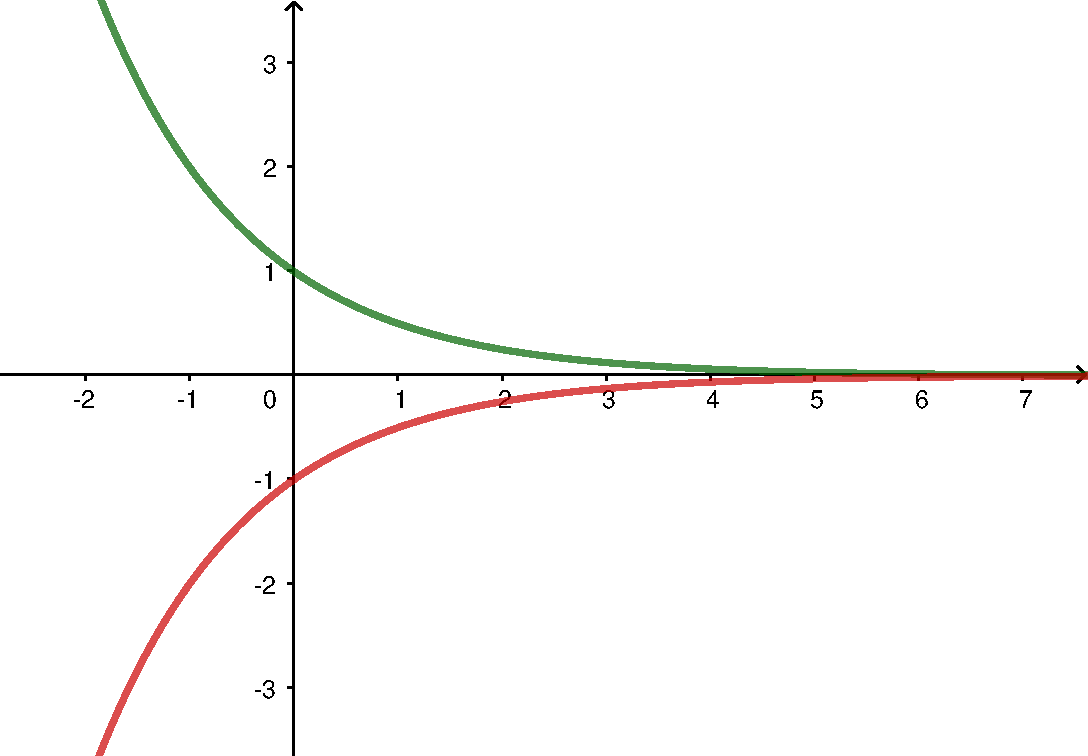
\includegraphics[scale=0.5]{immagini/cap3_Sistemi/sistEquilib.pdf}
%			\caption{ Grafico che descrive l'andamento della palla, come si può vedere tende a zero infatti il sistema è in equilibrio. }
%			\label{fig: funzbuca}
%		\end{figure}
	\end{nexample}
	
	\begin{nexample}
			Una palla che scivola da una collina è un esempio di sistema instabile, l'input è sempre la gravità e l'output è la velocità.
	
		\begin{figure}[H]
			\centering
%			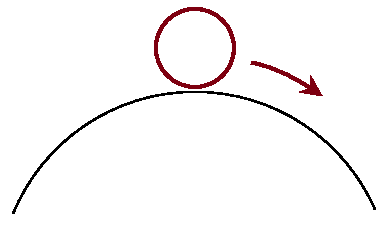
\includegraphics[scale=0.5]{immagini/cap3_Sistemi/pallaScivola.pdf}
%			\caption{ Sistema semplice: pendolo. }
			\subfloat[][\emph{Palla che scivola }]
			{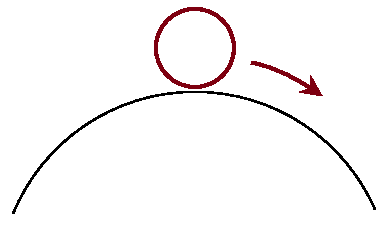
\includegraphics[width=.45\textwidth]{immagini/cap3_Sistemi/pallaScivola.pdf}} \quad
			\subfloat[][\emph{Grafico che descrive l'andamento della velocità di una palla che scivola, come si vede la velocità continuerà ad aumentare.}]
			{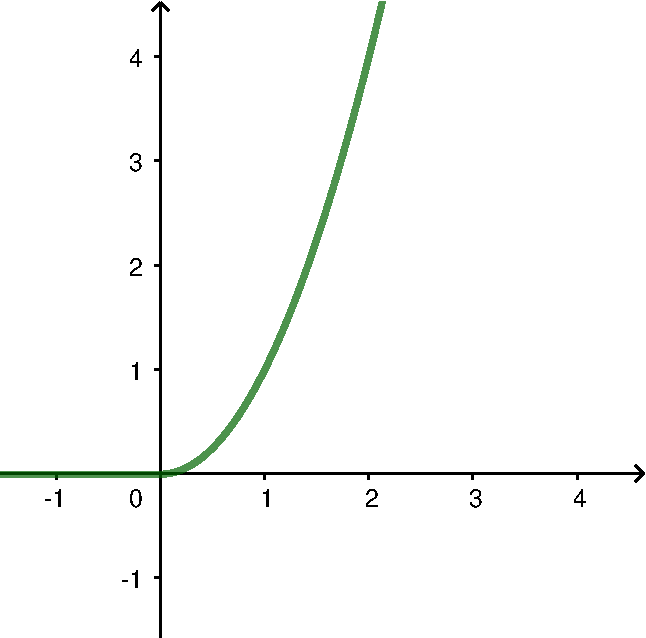
\includegraphics[width=.45\textwidth]{immagini/cap3_Sistemi/sistNonEquilib.pdf}} 
			\caption{ Sistema semplice: palla che scivola. }
			\label{fig: pallaScivola}
		\end{figure}
	
%		\begin{figure}[H]
%			\centering
%			\includegraphics[scale=0.5]{immagini/cap3_Sistemi/esp1Causale}
%			\caption{ Grafico che descrive l'andamento della velocità di una palla che scivola, come si vede la velocità continuerà ad aumentare. }
%			\label{fig: esp1Causale}
%		\end{figure}

	\end{nexample}
%%\pagebreak

%%%%%%%%%%%%%%%%%%%%%%%%%%%%%
%% Proprietà dei sistemi a tempo continuo
%%%%%%%%%%%%%%%%%%%%%%%%%%%%%

\section{Proprietà dei sistemi a tempo continuo}
	
	\subsection{Proprietà intrinseche: linearità, tempo invarianza e causalità}
	Con proprietà intrinseche intendiamo che i nostri sistemi per forza devono soddisfare queste proprietà.
		
		\subsubsection{Linearità}\label{sist_prop_Lin} 
		%TODO Aggiungere descrizione 
		%TODO immaigne: fare la formula come sistema a blocchi?
			\[
			\alpha u_1+\beta u_1 \overset{\text{sistema}}{\longmapsto} \alpha v_1+\beta v_2
			\]
			dove $ u_1 \overset{\text{sistema}}{\longmapsto} v_1$ e $u_2\overset{\text{sistema}}{\longmapsto} v_2$
			
		\subsubsection{Tempo invarianza} \label{sist_prop_TIn}
		%TODO Aggiungere descrizione 
		%TODO immaigne: fare la formula come sistema a blocchi?
			\[
			u(t-\tau) \overset{\text{sistema}}{\longmapsto} v(t-\tau)
			\]
			Se traslo nel tempo un segnale allora il segnale in uscita sarà traslato nel tempo della stessa quantità.
			
			\begin{definizione}
				I sistemi che soddisfano la linearità e la tempo invarianza li chiameremo sistemi LTI.
			\end{definizione}
		
		\subsubsection{Causalità (o non anticipatorio):} \label{sist_prop_cau}
			
			Con causalità si intende che l'effetto non precede la causa (la causa anticipa l'effetto).
			
			\begin{osservazione}
				Ci sarà sempre un istante iniziale $t_0$ a partire da cui studieremo il sistema.
			\end{osservazione}
		
			\[
				\exists \,t_0 \in \R \text{ tale che } u(t)=0 \text{ per } t<t_0
				\text{, allora } v(t)=0 \text{ per } t<t_0
			\]		
			Grazie alla tempo invarianza e alla causalità posso prendere per convenzione $ t_0 = 0$, cioè l'origine dell'evento.
			
%\pagebreak
		
			\begin{figure}[H]
				\centering
				\subfloat[][\emph{Sistema non causale}]
				{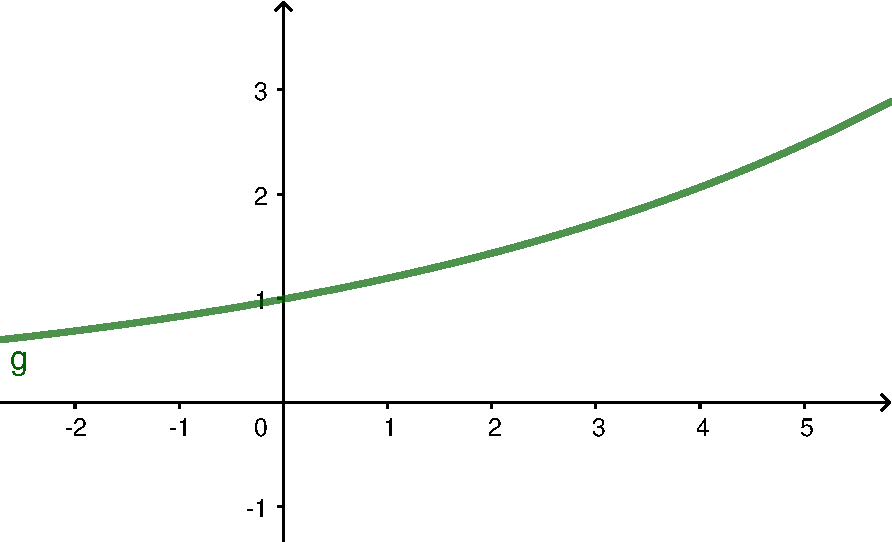
\includegraphics[width=.45\textwidth]{immagini/cap3_Sistemi/espNonCausale.pdf}} \quad
				\subfloat[][\emph{Sistema causale}]
				{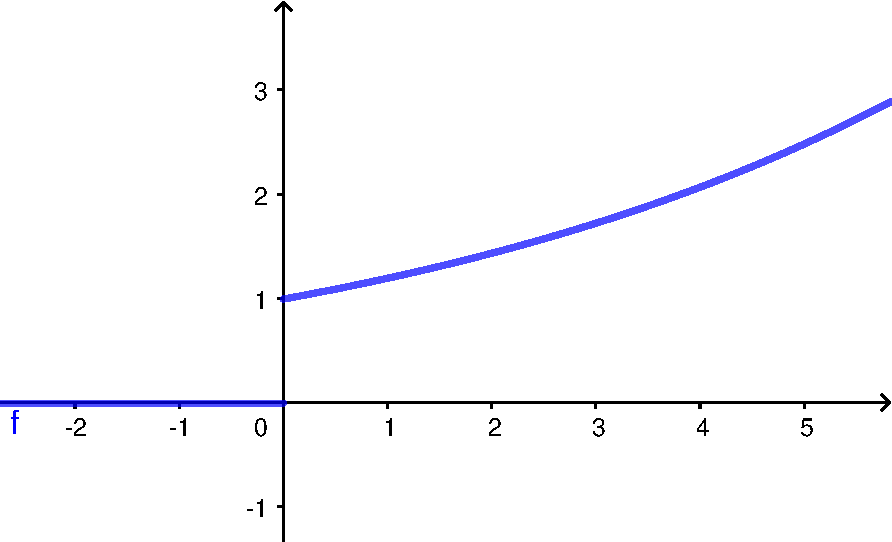
\includegraphics[width=.45\textwidth]{immagini/cap3_Sistemi/espCausale.pdf}} 
				\caption{ Esempio di sistema non causale e causale  }
				\label{fig: sistcausncaus}
			\end{figure}
			
%			\begin{figure}[H]
%				\centering
%				\includegraphics[scale=0.5]{}
%				\caption{ Sistema causale con $ t_0 = 0$. }
%				\label{fig: esp1Causale}
%			\end{figure}
	
	\subsection{Proprietà richieste: stabilità BIBO e stabilità asintotica}

		\subsubsection{Stabilità BIBO (bounded input bounded output)}\label{sist_prop_BIBOstab}
			
			Se l'entrate è limitata allora anche l'uscita sarà limitata (per sistemi causali).
			
			Scriviamo l'ingresso limitato come:
			\[
				\forall t \in [t_0, + \infty) \subseteq \R\text{, } \exists \, M_u >0 \text{ tale che } \lvert u(t) \rvert < M_u	
			\]
			
			Allora l'uscita limitata sarà:
				\[
			\exists \, M_v > 0 \text{ tale che } \forall t \in [t_0, + \infty) \text{, } \lvert v(t) \rvert < M_v
			\]
			%TODO aggiungere disegno
			
		\subsubsection{Stabilità asintotica}


			Se $\exists \, t_0 \text{ tale che } u(t)=0 \text{, } \forall t \ge t_0 \text{ allora } \lim_{t \to +\infty} v(t)=0$.\\
			In parole povere, in assenza di input l'output converge a zero asintoticamente: $\lim_{t \to \infty} v(t)=0$.
			
			\begin{NB}				
			La stabilità asintotica è più forte della BIBO, ovvero se trovo che un sistema è stabile asintoticamente so per certo che è anche BIBO stabile (non vale il contrario!).
			\end{NB}
			%TODO: aggiungere immagini?

%%%%%%%%%%%%%%%%%%%%%%%%%%%%%
%% Modelli
%%%%%%%%%%%%%%%%%%%%%%%%%%%%%
	
\section{Modelli descritti da equazioni differenziali}

\subsection{Esempi pratici}
\begin{nexample}
	Circuito elettrico
	
		\begin{figure}[H]
			\centering
			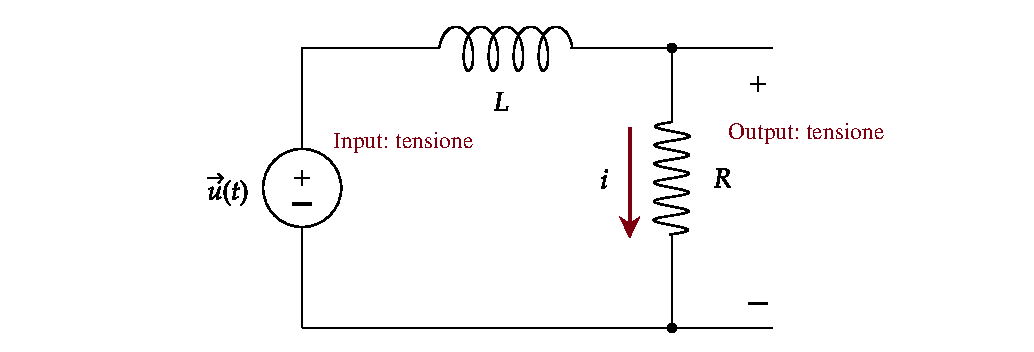
\includegraphics[scale=0.75]{immagini/cap3_Sistemi/circuito_RLC}
			\caption{ Circuito RLC. }
			\label{fig: circuito_RLC}
		\end{figure}
	 	In questo ambito L è l'induttanza (misurata in Henry) e R è la resistenza (misurata in Ohm). 
 	
	 	Per la legge di Kirchhoff trovo che: 
	 	\[ u(t) = L \frac{di(t)}{dt} + R i(t) \quad \text{e} \quad v(t) = R i(t) \]
	 	
	 	Allora avrò che $ \frac{L}{R} \frac{dv(t)}{dt} + v(t) = u(t)$ che posso riscrivere come:
	 	  \[ \frac{dv(t)}{dt} + \frac{R}{L} v(t) = \frac{R}{L} u(t) \]
	 	  
	 	Ho così modellato il sistema con un'equazione differenziale.
\end{nexample}

\begin{nexample}
	\label{es_mms}
	Sistema massa-molla-smorzatore 
	
		\begin{figure}[H]
			\centering
			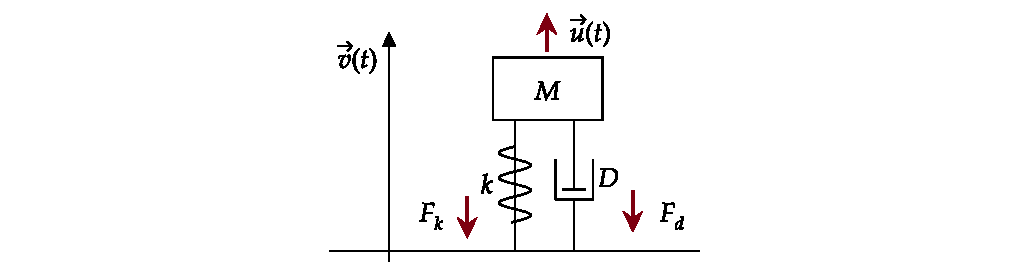
\includegraphics{immagini/cap3_Sistemi/massa_molla_smorzatore.pdf}
			\caption{ Sistema massa-molla-smorzatore. }
			\label{fig: massa_molla_smorzatore}
		\end{figure}
		
		In questo ambito Fk è la forza della molla (K costante elastica), Fd è la forza dello smorzatore (D costante di smorzamento), M è la massa, u(t) è la forza che applichiamo al sistema (l'input) e v(t) è lo spostamento nel tempo (l'output).
		
		\begin{NB}
			 v(t) è uno spostamento, non si intende una velocità! Quindi, solo in questo caso scriviamo: $ v(t) = x(t) $.
			Sapendo che $ F=ma $ e che $a= \frac{d^2 x(t)}{dt} $ abbiamo che:
			\[  M \frac{d^2 x(t)}{dt} = u(t) - F_d(t) - F_k(t) = u(t) - D \frac{d x(t)}{dt} - K x(t) \]
			con $ F_d $ e $ F_k $ forze opposte allo spostamento.
		\end{NB}
		
		Trovo anche qui una equazione differenziale che mi modella il sistema:
		\[  M x''(t) + D x'(t) + K x(t) = u(t) \]
		Sostituendo di nuovo avrò che:
		\[ M v''(t) + D v'(t) + K v(t) = u(t) \]
\end{nexample}


\subsection{Modelli SISO}

	In generale un modello SISO è descritto da un'equazione differenziale a coefficienti costanti di ordine $ n $.
	\begin{multline}
		a_n \frac{d^{(n)} v(t)}{dt^n} 
			+ a_{n-1} \frac{d^{(n-1)} v(t)}{dt^{n-1}} 
			+ \dots 
			+ a_1 \frac{dv(t)}{dt} 
			+ a_0\,v(t)\\
		= b_m \frac{d^{(m)} u(t)}{dt^m}
			+ b_{m-1} \frac{d^{(m-1)} u(t)}{dt^{m-1}} 
			+ \dots
			+ b_1 \frac{du(t)}{dt} 
			+ b_0\,u(t)
	\tag{2}\label{equation 2}
	\end{multline}
	con $ a_n, b_m \ne 0 $ ( Si ricorda che la parte a sinistra dell'uguale è l'output mentre quella a destra è l'input).
	
	Ricordiamo qui, per comodità, la prima equazione vista, cioè:
	\begin{equation*}
		\sum\limits_{i=0}^n a_{i} \frac{ d^{i} v }{ dt^{i}  } = \sum\limits_{i=0}^m b_{i} \frac{ d^{i} u }{ dt^{i}  }
		\tag{\ref{equation 1} rev.}
	\end{equation*}

	\begin{osservazione}
		Nei casi pratici, cioè in un sistema fisico, avrò che $n \ge m$.
	\end{osservazione}

	\begin{nexample}
		dall'esempio \ref{es_mms} di prima:
		 \[ M v''(t) + D v'(t) - K v(t) = u(u) \]
		quindi abbiamo che $ n = 2 $ e $ m = 0 $.
	\end{nexample}

	
	\begin{definizione}
		I sistemi in cui $n \ge m$ si chiamano \textbf{propri}.
		Se $n > m$ il sistema si chiamerà \textbf{strettamente proprio}.
	\end{definizione}
	
	\begin{osservazione}
		In generale l'uscita $v(t)$ del sistema (\ref{equation 1}) non è univoca.
		Se definiamo $n$ \textbf{condizioni iniziali} all'istante $t_0 = 0^-$ (per l'uscita $v$):
		\begin{equation}
			v(0^-) \,
			,\, \frac{dv(t)}{dt}\bigg\vert_{t=0^-} \,
			,\, \dots\,
			,\, \frac{d^{(n-1)}v(t)}{dt^{n-1}}\bigg\vert_{t=0^-}
			\tag{3}\label{equation 3}
		\end{equation}
		allora la soluzione di (\ref{equation 1}) è unica.
	\end{osservazione}
	
\subsection{Soluzione dei modelli SISO (evoluzione libera e forzata)}
	
	La soluzione dell'equazione (\ref{equation 1}) si ottiene come somma fra:
	\begin{itemize}
		\item una soluzione che dipende soltanto dalle condizioni iniziali (\ref{equation 3}) chiamata \textbf{evoluzione libera} con simbolo $v_l(t)$.
		\item una soluzione che dipende soltanto dall'ingresso $u(t)$ con condizioni iniziali tutte nulle, chiamata \textbf{ evoluzione forzata} con simbolo $v_f(t)$.
	\end{itemize}
	Avremo, cioè, che la soluzione dell'equazione (\ref{equation 1}) è:\\
	\[
	v(t) = v_l(t) + v_f(t)
	\]
	
\section{Evoluzione libera $ \rightarrow $ codizioni iniziali}
	L'evoluzione libera si ottiene dall'equazione dell'\textbf{omogenea associata}
	\begin{equation}
		a_n \frac{d^{(n)} v(t)}{dt^n} 
			+ a_{n-1} \frac{d^{(n-1)} v(t)}{dt^{n-1}} 
			+ \dots 
			+ a_1 \frac{dv(t)}{dt} 
			+ a_0\,v(t)
		= 0
		\tag{4}\label{equation 4}
	\end{equation}
	e le condizioni iniziali (\ref{equation 3}).
	
	Associamo a (\ref{equation 4}) l'\textbf{equazione caratteristica}:
	\begin{equation}
		a_n s^n 
		+ a_{n-1} s^{n-1}
		+ \dots
		+ a_1 s^1
		+ a_0 = 0
		\tag{5}\label{equation 5}
	\end{equation}
	con $a_n s^n + a_{n-1} s^{n-1} + \dots + a_1 s^1 + a_0 $ polinomio caratteristico.\\

	Sappiamo che per il toerema fondamentale dell'algebra, l'equazione (\ref{equation 5}) ha $r$ radici  distinte: $\lambda_1,\lambda_2, \dots, \lambda_r$ di molteplicità $\mu_1, \mu_2, \dots,\mu_r$ dove  $\mu_1 +\mu_2 + \dots + \mu_r = n$.
	
	La soluzione di (\ref{equation 4}) sarà:
	\begin{equation}
		v_\l(t)=  \sum_{i=1}^{r}\sum_{\l=0}^{\mu_i-1}c_{i,\l} \,e^{\lambda_it}\frac{t^\l}{\l!}
		\tag{6}\label{equation 6}
	\end{equation}
	con i coefficienti $c_{i,\l} $ che hanno indici $ i=\overline{1,r} $ e $ \l=\overline{o,\mu_{i-1}}$, $ \forall\mu_i \in \{\mu_1,\mu_2,\dots,\mu_r\} $. I coefficienti verranno determinati dalle condizioni iniziali (\ref{equation 3}).
		
	\begin{osservazione}
		Se $\mu_1 = \mu_2 = \dots = \mu_r = 1$ allora:
		\begin{equation*}
			v_l(t)=  \sum_{i=1}^{n}c_{i} \,e^{\lambda_it}
		\end{equation*}
		In cui mancano sia la seconda sommatoria sia $ \frac{t^\l}{\l!}$.
	\end{osservazione}
	
	\begin{definizione}
		$\displaystyle m(t) = e^{\lambda_i t} \frac{t^\l}{\l!} $ si chiama \textbf{modo elementare} del sistema.
	\end{definizione}
	\begin{nexample}
	L'equazione caratteristica è $ s^3 + 3 s^2 + 3s +1=0$
	
	Si ha che $ (s+1)^3=0$, avremo $ \lambda_{1} = -1$ con $ \mu_1=3 $. 
	Possiamo quindi scrivere la risposta libera come:
	\[ v_\l(t) =\sum_{i=1}^{r}\sum_{\l=0}^{\mu_i-1}c_{i,\l} \,e^{\lambda_it}\frac{t^\l}{\l!} \]
	Abbiamo, però, solo una radice quindi la prima sommatoria se ne va e rimane:
	 \[ v_\l(t) =\sum_{\l=0}^{3-1}c_{1,\l} \,e^{-1 t}\frac{t^\l}{\l!}  \]
	 \[ = c_{1,0} \, e^{-1t} + c_{1,1}\, e^{-1t} t + c_{1,2}\, e^{-1t} \frac{t^2}{2} \]
	\end{nexample}
	
	\begin{nexample}
	L'equazione caratteristica è $ (s+2)^2(s+1)^3=0 $
	
	Avrò quindi che $ \lambda_{1} = -2 $ con $ \mu_1=2 $ e $ \lambda_{2} = -1 $ con $ \mu_2=3 $.\\
	\[  v_\l(t) =\sum_{i=1}^{2}\sum_{\l=0}^{\mu_i-1}c_{i,\l} \,e^{\lambda_it}\frac{t^\l}{\l!} \]
	 \[ = c_{1,0}\, e^{-2t} + c_{1,1}\, e^{-2t} t + c_{2,0}\, e^{-t} + c_{2,1}\, e^{-t} t + c_{2,2}\, e^{-t} \frac{t^2}{2} \]
	\end{nexample}


	\begin{theorem}
		Dato un modo elementare $m(t) = e^{\lambda t} \frac{t^\l}{\l!} $ con $ \l \in \Z_+$, $ t \in \R$ e $ \lambda \in \C $.\\
		Abbiamo che:
		\begin{description}		
		\item[a)] $\Re( \lambda ) < 0 \Leftrightarrow  \lim_{t \to \infty} \, m(t) = 0 $.
		\item[b)] $\Re( \lambda ) \leq 0 \Leftrightarrow  m(t)$ limitato su $ [0, + \infty) $ e se $ Re( \lambda ) = 0 $ e $ \l=0$.
		\item[c)] in tutti gli altri casi ( cioè $ \Re( \lambda ) > 0 $ oppure $ \Re( \lambda ) = 0 $ e $ \l \neq 0$ ), $ \lim_{t \to \infty} m(t) = \infty $.
		\end{description}
	
		\begin{proof}[Dim]
		dimostriamo per casi.
		
		Sappiamo che $ \lambda \in \C$ quindi possiamo scriverlo anche come $ \lambda = \sigma + j \omega$ con $ \sigma = Re( \lambda)$.\\
		Possiamo quindi riscrivere il limite:
		 \[ \lim_{t \to \infty} m(t) = \lim_{t \to \infty} e^{\lambda t} \frac{t^\l}{\l!}= \lim_{t \to \infty} e^{(\sigma + j \omega ) t} \frac{t^\l}{\l!}= \lim_{t \to \infty} e^{\sigma t} e^{ j \omega t} \frac{t^\l}{\l!} \]
		\begin{description}	
		\item[c)] $ \sigma > 0$
		
		Allora $\displaystyle \lim_{t \to \infty} e^{\sigma t} e^{ j \omega t} \frac{t^\l}{\l!} = + \infty $ (il primo e il terzo tendono a $ \infty$, il secondo è limitato).
		Stessa cosa con $ \sigma = 0 $ e $ \l \neq 0 $ (il terzo tende a $ \infty$, il secondo è limitato, il primo tende a 1).
		
		\item[b)] $ \sigma > 0$ e $ \l =0$
		
		Allora $\displaystyle \lim_{t \to \infty} \frac{t^\l}{\l!} e^{\sigma t} e^{ j \omega t}$, il primo e il secondo tendono a 1, quindi possiamo scrivere il terzo argomento come $ \lim_{t \to \infty} ( \cos (\omega t) + j \sin (\omega t)) $.
		
		Il limite quindi non esiste ma è limitato tra -1 e 1.
		
		\item[a)] $ \sigma < 0$
		
		Allora $\displaystyle \lim_{t \to \infty} \frac{t^\l}{\l!} e^{\sigma t} e^{ j \omega t} = \lim_{t \to \infty} \frac{t^\l }{\l! e^{-\sigma t}}  e^{ j \omega t} = 0$ (la forma è indeterminata $\displaystyle \frac{\infty}{\infty}$, vince quello sotto).
	\end{description}	
		\end{proof}
	\end{theorem}

%%%%%%%%%%%%%%%%%%%%%%%%%%%%%
%% Stabilità asintotica
%%%%%%%%%%%%%%%%%%%%%%%%%%%%%

\section{Stabilità asintotica}
	
	Si studia la stabilità asintotica di sistemi descritti dall'equazione:
	\begin{equation*}
	\sum\limits_{i=0}^n a_{i} \frac{ d^{i} v }{ dt^{i}  } = \sum\limits_{i=0}^m b_{i} \frac{ d^{i} u }{ dt^{i}  }
	\tag{\ref{equation 1} rev.}
	\end{equation*}

	
	Dal teorema visto prima ne enunciamo un altro di maggiore importanza.
	
	\begin{theorem}
		il sistema (\ref{equation 1}) è asintoticamente stabile se per ogni scelta delle condizioni iniziali (\ref{equation 3}):
		\begin{equation*}
			\lim_{t \to \infty}v_\l(t)=0
			\Leftrightarrow\text{tutti i modi elementari } m(t)=e^{\lambda t}\frac{t^\l}{\l!}\text{ sono convergenti a $0$}
			\Leftrightarrow \Re(\lambda_i)<0,\forall i = \overline{1,r}
		\end{equation*}
	\end{theorem}
	\begin{nexample}
	Analizziamo la stabilità del circuito elettrico
	
	Abbiamo visto che il circuito elettrico RLC è modellato da:
	 \[ \frac{dv(t)}{dt} + \frac{R}{L} v(t) = \frac{R}{L} u(t) \]
	L'equazione caratteristica è $ s + \frac{R}{L}=0 $ con s numero complesso.
	Ho un'unica radice che risolve l'equazione ed è $ \lambda = - \frac{R}{L}$ con $ R > 0$ e $ L > 0$.
	
	$\Re(\lambda) = - \frac{R}{L}$ e noi vogliamo che sia negativa (dal teorema precedente). Visto che ho $ R > 0$ e $ L > 0$, allora il sistema sarà sempre stabile.
	\end{nexample}

	\begin{nexample}	
	Calcoliamo la risposta libera del sistema massa-molla-smorzatore.
	
	Abbiamo visto che questo sistema è modellato da:
	 \[ M v''(t) + D v'(t) - K v(t) = u(t) \]
	con $ M, D, K>0 $.
	
	L'equazione caratteristica è $ M s^2 + Ds + K=0 $ con s numero complesso.
	
	Le radici saranno $\displaystyle \lambda_{1,2} = \frac{-D\pm \sqrt{D^2 - 4KM}}{2M}$.
	\begin{itemize}
		\item Se $ \lambda_{1} \neq \lambda_{2} $ allora la risposta libera è $ v_\l(t) = C_{1,0}\, e^{\lambda_{1}t} + C_{2,0}\, e^{\lambda_{2}t}$.
		\item Se $ \lambda_{1} = \lambda_{2} $ allora la risposta libera è $ v_\l(t) = C_{1,0}\, e^{\lambda_{1}t} + C_{1,1}\, e^{\lambda_{1}t} $.
	\end{itemize}
	\end{nexample}


%%%%%%%%%%%%%%%%%%%%%%%%%%%%%
%% Convoluzione
%%%%%%%%%%%%%%%%%%%%%%%%%%%%%

\section{Convoluzione}
	
	\begin{definizione}
		Date due funzioni $v_1(t)$ e $v_2(t) $ con $ t\in\mathbb{R} $ definiamo il prodotto (o integrale) di \textbf{convoluzione} come:
		\begin{equation*}
			(v_1 * v_2)(t_0) 
			= \int_{-\infty}^{\infty}v_1(\tau)v_2(t_0 - \tau)\d\tau 
			= \int_{-\infty}^{\infty}v_1(t_0 - \tau)v_2(\tau )\d\tau
		\end{equation*}
		con $t_0 $ fissato.
	\end{definizione}
		
	Proprietà della convoluzione:
		\begin{enumerate}
			\item $v_1 * v_2 = v_2 * v_1 $ (commutatività)
			\item $(v_1 * v_2) * v_3  = v_1 * (v_2 * v_3) $ (associatività)
			\item $v_1 * (v_2 + v_3)  = v_1 * v_2 + v_1 * v_3$ (distributività rispetto alla somma)
		\end{enumerate}
		Queste proprietà sono immediate, per dimostrarle sostituisco con gli integrali.
	
	\begin{osservazione}
		\textbf{Proprietà di riproducibilità dell'impulso}
		
		L'elemento neutro della convoluzione è $ \delta(t)$.
		\[ (v *\delta)(t)\overset{def}{=} \int_{-\infty}^{\infty}v(\tau)\delta(t - \tau)\d\tau = v(t) \]
	\end{osservazione}
	
	Dimostrazione fatta con il sistema a box (guarda gli appunti). %TODO: riferimento a cosa?
	%TODO: se hai voglia fallo
		
%%%%%%%%%%%%%%%%%%%%%%%%%%%%%
%% Risposta impulsiva
%%%%%%%%%%%%%%%%%%%%%%%%%%%%%

\section{Risposta impulsiva}
	
	\begin{definizione}
		Dato un sistema descritto dall'equazione (\ref{equation 1}), inizialmente a riposo, definiamo la \textbf{risposta impulsiva} l'uscita del sistema in corrispondenza dell'impulso unitario $\delta (t)$ in ingresso. La indichiamo con $h(t)$.
	\end{definizione}
	
	\textbf{In parole semplici: }
	\begin{enumerate}
	\item Posso calcolare la risposta impulsiva $ h(t) $  definita come l'uscita con ingresso un impulso $\delta(t)$.
	\item Grazie ad esso posso trovare l'uscita di un sistema facendo la convoluzione fra l'ingresso e $ h(t) $.
	\end{enumerate}

	\textbf{In dettaglio: } 
		
	Tenendo conto che $h(t)=0$ per $t<0$ (causalità) avremo:
	\begin{equation*}
	v(t)= \int_{0^-}^{\infty}h(\tau)u(t - \tau)\d\tau 
	= \int_{-\infty}^{t^+}h(t - \tau)u(\tau)\d\tau
	\end{equation*}
	Tutto ciò è dovuto sostituiendo:  $t-\tau = s \Rightarrow d\tau = - ds 
	\qquad \tau = 0^-  \Rightarrow s = t^+ 
	\qquad \tau=\infty \Rightarrow s = -\infty$
	
	Ora è possibile cambiare gli estremi dell'integrale con un cambio di segno.
	\[
	\int_{t^+}^{\infty}h(t-s)u(s)\,-ds 
	=-\int_{t^+}^{\infty}h(t-s)u(s)\d s
	=\int_{-\infty}^{t^+}h(t-s)u(s)\d s
	\qedhere
	\]
	
	La risposta in uscita del sistema (\ref{equation 1}), inizialmente a riposo, di risposta impulsiva $h(t)$ con $ t\in\R$ in corrispondenza a un ingresso $u(t)$, se esiste, è data da:
	\[
	v(t)=(h*u)(t) = \int_{0^-}^{\infty}h(\tau)u(t - \tau)\d\tau
	= \int_{-\infty}^{t^+}h(t - \tau)u(\tau)\d\tau
	\]
	
	\begin{NB}
	 Sostituendo $\delta (t)$ in (\ref{equation 1}), la risposta impulsiva caratterizza il sistema (cioè le sue proprietà):
	\begin{equation}
		a_n\frac{d^{(n)}h(t)}{dt^n}+\dots+a_0\,h(t)
		=b_m\frac{d^{m}\delta(t)}{dt^{m}}+\dots+b_0 \delta(t)
	\tag{7}\label{equation 7}
	\end{equation}
	\end{NB}:
%%%%%%%%%%%%%%%%%%%%%%%%%%%%%
%% Evoluzione forzata
%%%%%%%%%%%%%%%%%%%%%%%%%%%%%

\section{Evoluzione forzata $ \rightarrow $ ingresso u(t)}

	Posso calcolare la \textbf{risposta forzata} ad un ingresso $u(t)$ con $ t\in\R $ grazie alla risposta impulsiva h(t). $ u(t)=0 $ quando $ t<0$ (causalità).
	
	La risposta forzata è:	
	\[
	v\!_f(t) =
	\int_{0^-}^{t^+}h(t - \tau)u(\tau)\d\tau 
	\,= 
	\int_{0^-}^{t^+}h(\tau)u(t - \tau)\d\tau 
	\]
	
	Studiamo ora l'evoluzione forzata sull'orizzonte temporale $(0^+,+\infty)$.
	\begin{equation*}
		h(0) = \frac{dh(t)}{dt}\bigg\vert_{t=0^-} = \dots 
		=\frac{d^{(n-1)}h(t)}{dt^{n-1}}\bigg\vert_{t=0^-}
		= 0
	\end{equation*}
	
	\begin{NB}
		 $ \delta(t) = 0$ per $ t >0$ (vedi definizione di delta).
	\end{NB}

	\begin{equation}
	 a_n \frac{d^{n} h(t)}{dt^n}+\dots+a_0\,h(t) = 0
	\tag{8}\label{equation 8}
	\end{equation}
	È un equazione differenziale omogenea. Si noti:
	\begin{itemize}
		\item Per $ t\leq0 $, ho la risposta libera (influenzata dalle condizioni iniziali).
		\item Per $ t>0 $, ho la risposta forzata (influenzata dall'ingresso).
	\end{itemize}

	\begin{osservazione}
		Dalla (\ref{equation 8}) vediamo che $ h(t) $ è una combinazione lineare di tutti i modi elementari ottenuti dalla soluzione dell'equazione caratteristica del sistema (\ref{equation 1}) in cui si aggiunge un termine impulsivo soltanto nei sistemi in cui $n=m$ (lo vedremo meglio più avanti):
		\begin{equation}
			 h(t)= d_0 \delta(t) + \sum_{i=1}^{r}\sum_{\l=0}^{\mu_i-1}d_{i,\l} \,e^{\lambda_it}\frac{t^\l}{\l!}\delta_{-1} (t)
			\tag{9}\label{equation 9}
		\end{equation}
		dove $ d_0 \delta(t) $ è il termine impulsivo quando $ n=m$ e $ \sum_{i=1}^{r}\sum_{\l=0}^{\mu_i-1}d_{i,\l} \,e^{\lambda_it}\frac{t^\l}{\l!}\delta_{-1} (t) $ è la combinazione lineare dei modi elementari (da notare che $C_{i,\l}\neq d_{i,\l} $, i coefficienti non sono gli stessi della risposta libera ).
	\end{osservazione}
	
	\begin{NB}
		se $h(t)=0 $ con $ t<0$ (causalità) allora $h(t) = h(t)\delta_{-1} (t)$.
	\end{NB}

\begin{nexample}

	determina la risposta impulsiva $ h(t $) del sistema:
	\[ \frac{dv(t)}{dt} + 2v(t) = \frac{du(t)}{dt} + u(t) \]
	\begin{NB}
		Siamo nel caso $n=m$.
	\end{NB}
	
	L'equazione caratteristica è $ s+2=0$ e la radice che la risolve è $ \lambda = -2$.
	Il modo elementare è $ m(t) = e^{-2t} $.
	
	Allora la risposta impulsiva sarà:
	\[ 
		h(t) = d_0 \delta (t) + d_1 e^{-2t} \delta_{-1}(t)  
	\]
	Ora vogliamo trovare $ d_0 $ e $ d_1 $, per fare ciò dobbiamo derivare la risposta impulsiva quindi avremo:\\
	\[ 
		\frac{d h(t)}{dt} 
		= d_0 \frac{d \delta (t)}{dt} 
		- 2 d_1 e^{-2t} \delta_{-1}(t)
		+ d_1 e^{-2t} \delta(t) 
	 \]
	Notiamo che $\displaystyle	e^{-2t} \delta (t) = e^{-2t}\big\vert_{t=0} \delta (t)= \delta (t) $. Sostituiamo dentro a:
	\[
		\frac{dv(t)}{dt} + 2v(t) = \frac{du(t)}{dt} + u(t) \qquad v(t) \rightarrow h(t) \text{ e }  u(t) \rightarrow \delta (t) 
	\]
	Verrà che  
	\[ 
		d_0 \frac{d \delta (t)}{dt} 
		- 2 d_1 e^{-2t} \delta_{-1}(t)
		+ d_1 \delta(t)
		+2 [d_0 \delta (t) + d_1 e^{-2t} \delta_{-1}(t) ]
		= \frac{d \delta (t)}{dt} + \delta (t) 
	\]
	Sempre per lo stesso motivo $\displaystyle e^{-2t} = e^{-2t}\big\vert_{t=0} = 0$, si semplifica: 
	\[
 		d_0 \frac{d \delta (t)}{dt}
		+ d_1 \delta(t)
		+2 d_0 \delta (t)
		= \frac{d \delta (t)}{dt} + \delta (t) 
	\]
	
	Si porta a sinistra tutto e si raggruppa $\frac{d \delta (t)}{dt}$ e $ \delta (t) $:
	\[
		(d_0-1) \frac{d \delta (t)}{dt}
		+ (d_1 + 2 d_0 -1) \delta(t) =0  
	\]
	\[
 		\begin{cases} 
			d_0 -1=0 \rightarrow d_0=1 \\ 
			d_1 + 2 d_0 -1 = 0 \rightarrow d_1 = -1
		\end{cases} 
	\]
	
\end{nexample}	


%%%%%%%%%%%%%%%%%%%%%%%%%%%%%
%% Sistemi LTI generali definiti dalla risposta impulsiva
%%%%%%%%%%%%%%%%%%%%%%%%%%%%%

\section{Sistemi LTI generali definiti dalla risposta impulsiva (non causali)}
	
	Per i sistemi causali abbiamo $h(t) =0$ con $ t<0$, ma in generale possiamo descrivere un sistema SISO associando ad un ingresso $u(t)$ con $ t \in \R$ (non più quindi $t>0$) e ad una funzione $h(t)$, l'uscita:
	\begin{equation}
		v(t)=(h*u)(t) = \int_{-\infty}^{+\infty}h(\tau)u(t-\tau)\d\tau
		\tag{10}\label{equation 10}
	\end{equation}
	
	\begin{NB}
	$h(t)=(h* \delta )(t)$, cioè la delta è l'elemento neutro della convoluzione.
	\end{NB}	

	Per i sistemi LTI causali:
	\[
		v(t)=(h*u)(t) = \int_{-\infty}^{t^+}h(t-\tau)u(\tau)\d\tau = \int_{0^-}^{+\infty}h(\tau)u(t-\tau)\d\tau
	\]
	Rispetto a (\ref{equation 10}) non ho $ (-\infty...+\infty)$ ma $ (-\infty...t^+)$ o $ (0^-...+\infty)$ perchè ora ho sistemi causali.

%%%%%%%%%%%%%%%%%%%%%%%%%%%%%
%% Stabilità BIBO dei sistemi LTI generali
%%%%%%%%%%%%%%%%%%%%%%%%%%%%%
	
\section{Stabilità BIBO dei sistemi LTI generali}
	\label{sec:BIBO}
	
	Riprendiamo la definizione di BIBO stabilità:
	
	se si ha un ingresso limitato $ | u(t) |  < M_u$, $ \forall t \in \R$,	allora esiste $ M_v $ tale che $| v(t) | < M_v $ con $ \forall t \in \R $, cioè abbiamo un'uscita limitata.
	
	\subsubsection{Proprietà}
	Un sistema a tempo continuo LTI è BIBO stabile se e solo se:
	\[
		\int_{-\infty}^{+\infty}\lvert h(t) \rvert \d t < +\infty
	\]
	cioè la risposta impulsiva è sommabile oppure assolutamente integrabile.
	
	Dimostriamo ora $\Leftrightarrow $, quindi prima $\Leftarrow $ e dopo $ \Rightarrow$.
	\begin{proof}[Dim]
		\emph{$(\Leftarrow)$}
		\[
			\int_{-\infty}^{+\infty}\lvert h(t) \rvert \d t < +\infty \quad \overset{?}{\Rightarrow} \quad \text{BIBO stabile}
		\]	
		Dato un ingresso $u(t) $ tale che $ \lvert u(t) \rvert < M_u , \forall t \in \R$. Dobiamo dimostrare che $ v(t) $ sia limitato per $ t \in \R $, cioè esiste $ M_v $ tale che $| v(t) | < M_v $ con $ \forall t \in \R $. 
		
		Sappiamo che 
		$\displaystyle
			v(t)
			=(h*u)(t) 
			= \int_{-\infty}^{+\infty}h(\tau)u(t-\tau)\d\tau 
		$:
		
		\[
			\abs{ v(t)} 
			= \bigg\lvert \int_{-\infty}^{+\infty}h(\tau)u(t-\tau)\d\tau \,  \bigg\rvert
			\le \int_{-\infty}^{+\infty} \rvert h(\tau)u(t-\tau) \lvert\d\tau
			= \int_{-\infty}^{+\infty} \rvert h(\tau) \lvert \, \underbrace{\rvert u(t-\tau) \lvert}_{\le M_u} \d\tau
		\]
		
		\[
			\le \int_{-\infty}^{+\infty} \rvert h(\tau)\lvert M_u \d\tau 
			= M_u \int_{-\infty}^{+\infty} \rvert h(\tau)\lvert  \d\tau
		\]
		
		La nostra ipotesi ci dice che $ \int_{-\infty}^{+\infty} \rvert h(\tau)\lvert  \d\tau < + \infty$.
		Scegliendo $ M_v \coloneqq M_u \int_{-\infty}^{+\infty} \rvert h(\tau)\lvert\d\tau \in \mathbb{R}$\\
		allora $ \lvert v(t) \rvert < M_v, \forall t \in \mathbb{R}$
		di conseguenza il sistema è BIBO stabile.
	\end{proof}
	
	\begin{proof}[Dim]
		\emph{$(\Rightarrow)$}
		\[
			\text{BIBO stabile} \quad \overset{?}{\Rightarrow} \quad \int_{-\infty}^{+\infty}\lvert h(t) \rvert \d t < +\infty
		\]
		Per assurdo supponiamo che :
		\[
			\int_{-\infty}^{+\infty}\lvert h(t) \rvert \d t = +\infty
		\]
		
		Cerchiamo  una contraddizione partendo dalla BIBO stabilità:
		
		$\forall u(t)$ con $ |u(t)| <M_u $, abbiamo che esiste $ M_v$ tale che $ v(t) = (h*u)(t)$ con $ \lvert v(t) \rvert < M_v $ per ogni $ t \in \R$.
		
		Scegliamo:
		\[
			u(t) = \sng(h(-t)) = \begin{cases}
				1 &h(-t)>0\\
				0 &h(-t)=0\\
				-1 &h(-t)<0\\
			\end{cases}
		\]
		Quindi di sicuro $\lvert u(t)\rvert <2$, scegliamo $ M_u = 2$, cioè abbiamo l'ingresso limitato.
		
		Di conseguenza:
		\[
			t \in \R \quad v(t) = \int_{-\infty}^{+\infty}h(\tau)u(t-\tau)\d\tau 
		\]
		
		Per $t=0$:
		\[
			v(0) = \int_{-\infty}^{+\infty}h(\tau)u(-\tau)\d\tau 
			= \int_{-\infty}^{+\infty}\underbrace{h(\tau)\, \sng(\tau)}_{\lvert h(\tau)\rvert}\d\tau
			= \int_{-\infty}^{+\infty}\lvert h(\tau) \rvert \d\tau = +\infty
		\]
		Ci troviamo in contraddizione con l'ipotesi.
	\end{proof}
	
	\begin{osservazione}\leavevmode
		\begin{enumerate}
			%1
			\item Per i sitemi LTI causali: BIBO stabilità $\Leftrightarrow \int_{-\infty}^{+\infty}\lvert h(t) \rvert \d t < +\infty$
			
			%2
			\item Dato $ h(t)= d_0 \delta(t) + \sum_{i=1}^{r}\sum_{\l=0}^{\mu_i-1}d_{i,\l} \,e^{\lambda_it}\frac{t^\l}{\l!}\delta_{-1} (t)  $ per il sistema (\ref{equation 1})
			allora $h(t) $ è sommabile \\
			$\Leftrightarrow$ tutti i modi sono cenvergenti per $d_{i,\l}\ne0$\\
			$\Leftrightarrow \Re(\lambda_i)<0$\\
			$ \Leftrightarrow $ è BIBO stabile
			
			%3
			\item Se guardo i modi di$  h(t) $ come un'insieme\\
			\{I modi di $h(t)$\} $\subseteq$ \{i modi di $v_\l(t)$\} (perchè alcuni modi sono uguali a zero, $d_{i,\l}=0$ )
			
			%4
			\item  Stabilità asintotica $\Rightarrow$ BIBO stabilità (il contrario non è valido $\cancel{\Leftarrow}$ )
		\end{enumerate}
	\end{osservazione}

%%%%%%%%%%%%%%%%%%%%%%%%%%%%%
%% Risposta in frequenza
%%%%%%%%%%%%%%%%%%%%%%%%%%%%%

\section{Risposta in frequenza}
		
	%TODO: wikipedia ci dice che
	\textbf{Wikipedia:}\\
	La \textbf{risposta in frequenza o risposta armonica} di un sistema è la descrizione della sua uscita 
	(una funzione del tempo) utilizzando come variabile la frequenza invece che il tempo 
	(ovvero nel dominio della frequenza).
	
	L'analisi in frequenza del comportamento di un sistema viene svolta molto spesso 
	quando si ha a che fare con sistemi lineari (in configurazione stabile), 
	i quali hanno la fondamentale proprietà di rispondere ad un input puramente sinusoidale 
	con un'uscita della stessa frequenza, ovvero restituiscono la medesima sinusoide in ingresso, 
	ma sfasata e moltiplicata per un fattore scalare (amplificata). 
	Se il sistema è un sistema dinamico lineare stazionario (LTI) tale fattore moltiplicativo non varia 
	nel tempo; 
	per tale motivo la risposta in frequenza di sistemi LTI viene caratterizzata completamente 
	dalla risposta all'impulso, cioè dall'uscita del sistema quando in ingresso vi è un impulso
	a delta di Dirac. 
	La risposta in frequenza è in tal caso esplicitata dalla \textbf{funzione di trasferimento} 
	(definita come la trasformata di Laplace della risposta all'impulso a delta di Dirac).
	%TODO: FINE wikipedia ci dice che

	Con la risposta in frequenza, si cerca di analizzare l'uscita sistema usando come variabile di ingresso la frequenza al posto del tempo. Si passa, cioè, dal dominio del tempo a quello della frequenza.
	Questa analisi si usa principalmente con i sistemi lineari i quali rispondono ad un'entrata sinusoidale con un'uscita nella stessa frequenza. Cioè la sinusoidale in ingresso scalata nell'ampiezza e con una determinata fase. Se il sistema è LTI il fattore che modifica l'ampiezza non varia nel tempo.
	Per questo motivo la risposta ad un impulso di dirac, definita \textbf{funzione di trasferimento}, caratterizza completamente il sistema. 
	
	Guardiamo ora in dettaglio:
	
	Abbiamo ora un sistema generale quindi non causale.
	
	Dato un sistema LTI e BIBO stabile di risposta impulsiva $h(t)$ con $ t \in \R$ reale a valori reali, mi interessa la risposta in corrispondenza di \textbf{ingressi esponenziali con esponente immaginario puro (fasori)}.
	
	\[ 
		 u_1(t) =Ae^{j(\omega_0 t + \phi)}= Ae^{j\phi}e^{j\omega_0 t} \quad \overset{h(t)\text{ BIBO stabile}}{\longmapsto} \quad v_1(t)
	\]
	con $A \in \R_+, \phi$ e $\omega_0 \in \R$.
	
	Voglio sapere in dettaglio $ v_1(t)$.\\
	\[
		v_1(t) 
		= \int_{-\infty}^{+\infty}h(\tau)u_1(t-\tau)\d\tau
		= \int_{-\infty}^{+\infty}h(\tau)Ae^{j(\omega_0(t-\tau)+\phi)}\d\tau
		= Ae^{j(\omega_0 t+\phi)}
		\int_{-\infty}^{+\infty}h(\tau)e^{-j\omega_0 \tau} \d\tau
	\]
	Il sistema come da premessa è BIBO stabile quindi:
	\[ \int_{-\infty}^{+\infty}\lvert h(t) \rvert \d t < +\infty \]
	e la prima parte $ Ae^{j(\omega_0 t+\phi)} $ è un numero complesso (quindi non ci interessa e non lo consideriamo).\\
	Prendiamo l'integrale e mettiamolo in modulo:
	\[
		\Abs{\int_{-\infty}^{+\infty}h(\tau)e^{-j\omega_0 \tau}\d\tau} 
		\le \int_{-\infty}^{+\infty}\abs{h(\tau)e^{-j\omega_0 \tau}}\d\tau
		= \int_{-\infty}^{+\infty}\abs{h(\tau)}\abs{e^{-j\omega_0 \tau}}\d\tau
		= \int_{-\infty}^{+\infty}\abs{h(\tau)}\d\tau < +\infty
	\]
	visto che $\abs{e^{-j\omega_0 \tau}} =1$ (cioè il modulo di un fasore è sempre 1).\\
	Ora possiamo scrivere:
	\[
		H(j\omega_0) = \int_{-\infty}^{+\infty}h(\tau)e^{-j\omega_0 \tau}\d\tau
	\]
	\[
		\Rightarrow v_1(t)=H(j\omega_0) A e^{j(\omega_0 t + \phi)}, \quad t \in \R
	\]
	Abbiamo visto che questa $ H $ esiste perchè l'integrale di prima converge.
	
	\begin{definizione}
		La facciamo diventare una funzione, per $ \omega \in \mathbb{R} $ definiamo
		\[
			H(j\omega)= \int_{-\infty}^{+\infty}h(\tau)e^{-j\omega \tau}\d\tau
		\]
		e la chiamamo la \textbf{risposta in frequenza} del sistema (\ref{equation 10}).
	\end{definizione}
	

	\begin{definizione}
		se $ \forall\omega\in\R \mapsto H(j\omega)\in \C$, allora esistono due funzioni:
		\begin{itemize}
			\item $ A(\omega) $ chiamata \textbf{modulo o ampiezza}
			\item $ \Phi(\omega) $ chiamata \textbf{fase o argomento}
		\end{itemize}

		tali che:
		\begin{gather*}
			A(\omega)\coloneqq\abs{H(j\omega)}=\Abs{\int_{-\infty}^{+\infty}h(\tau)e^{-j\omega \tau}\d\tau}\\
			\Phi(\omega) \coloneqq \angle H(j\omega)=arg(H(j\omega))=arg(\int_{-\infty}^{+\infty}h(\tau)e^{-j\omega \tau}\d\tau)
		\end{gather*}
	\end{definizione}
	
	Definite queste due funzioni possiamo riscrivere $v_1(t) $ come:
	\[
		v_1(t) =(A(\omega_0)A)e^{j(\omega_0 t+\phi+\Phi(\omega_0))} , \quad t \in \mathbb{R}
	\]
	
	Se prendo $ u_2(t)= A e^{-j(\omega_0 t + \phi)}$:
	\[
		v_2(t)
		=H(-j\omega_0)Ae^{-j(\omega_0 t+\phi)}
		=A(-j\omega_0)Ae^{j(\omega_0 t+\phi+\Phi(-\omega_0))}
	\]
	\[
		H(-j\omega_0)
		=\int_{-\infty}^{+\infty}\underbrace{h(\tau)}_{\in\R}e^{j\omega \tau}\d\tau
		= \int_{-\infty}^{+\infty}\overline{h(\tau)e^{-j\omega \tau}}\d\tau
		= \overline{\int_{-\infty}^{+\infty}h(\tau)e^{-j\omega \tau}\d\tau}
		= \overline{H(j\omega_0)}
	\]
	
	Quindi $ H(-j\omega_0)= \overline{H(j\omega_0)}$, cioè il complesso coniugato.
	
	\begin{itemize}
		\item	$ A(j\omega) =A(-j\omega)$. L'ampiezza è pari, cioè ho la stessa ampiezza tra complesso e il suo coniugato.
		\item $ \Phi(j\omega) =-\Phi(-j\omega)$. La fase è dispari, cioè ho la fase opposta tra complesso e il suo coniugato.
	\end{itemize}
	
	Supponiamo ora un ingresso $ u(t)=A \cos(\omega_0 t+\phi), \quad t \in \mathbb{R},\quad A>0, \quad \omega_0 \text{ e } \phi \in \mathbb{R} $.\\
	
	Con la formula di Eulero diventa:
	
	\begin{equation*}
		u(t)=\frac{A}{2}e^{j(\omega_0 t + \phi)}+\frac{A}{2}e^{-j(\omega_0 t + \phi)} 
			= \frac{u_1(t)+ u_2(t)}{2}
	\end{equation*}
	\begin{equation*}
		\Rightarrow v(t)=
			\frac{v_1(t)+ v_2(t)}{2}
			= \frac{A e^{j(\omega_0 t + \phi)}  H(j\omega_0)+ A e^{-j(\omega_0 t + \phi) }H(-j\omega_0)}{2}
	\end{equation*}
	
	essendo complesso coniugato:
	\begin{equation*}
			= \frac{A e^{j(\omega_0 t + \phi)} A(\omega_0) e^{j\Phi(\omega_0)} + A e^{-j(\omega_0 t + \phi)} A(\omega_0) e^{-j\Phi(\omega_0)}}{2}\\
	\end{equation*}
	
	Applicando la formula di Eulero al contrario:
	\begin{equation*}
	=A A(\omega_0)cos(\omega_0 t+\phi+\Phi(\omega_0))
	\end{equation*}
	Ho quindi sempre un coseno (come detto prima) ma amplificato e sfasato.
	
	La risposta di un sistema LTI reale ($ h(t) $ reale) e BIBO stabile a un segnale sinusoidale di frequenza $ \omega_0 $ è ancora un segnale della stessa frequenza:
	
	\begin{enumerate}	
	\item L'ampiezza è data dal prodotto dell'ampiezza dell'ingresso A e il modulo della risposta in frequenza:
	\begin{equation*}
		A \abs{H(j\omega_0)}=AA(\omega_0)
	\end{equation*}
	\item La fase è data dalla fase iniziale $ \phi $ sommata alla fase della risposta in frequenza:
	\begin{equation*}
		\angle H(j\omega) = \phi + arg(H(j\omega_0)) = \phi + \Phi(\omega_0)
	\end{equation*}
	\end{enumerate}

	In conclusione, per il sistema (\ref{equation 1}):
	\[
		u(t)= e^{j\omega t}
		\Rightarrow v(t) = e^{j\omega t} H(j\omega)
	\]
	dove  $ H(j\omega) $ è la risposta in frequenza.
	
	Ricordiamo che:
	\[
		\frac{d^{(i)}e^{j\omega t}}{dt^i} = (j\omega)^i e^{j\omega t}
	\]
	inseriamo in (\ref{equation 1}): 
	\[
		\sum_{i=0}^{n}a_i\, H(j\omega)(j\omega)^i \cancel{e^{j\omega t}}
		= \sum_{i=0}^{m}b_i \, (j\omega)^i \cancel{e^{j\omega t}}
	\]
	\[
		\Rightarrow H(j\omega) = \frac{\sum_{i=0}^{m}b_i \, (j\omega)^i}{\sum_{i=0}^{n}a_i\, (j\omega)^i}
	\]
	Quest'ultima ci risulterà molto utile in seguito.



